% Methodology
% Generated by report/md2tex.py from Report.md -- edit Report.md, then re-run.

\section{Methodology}

\subsection{Pipeline architecture}

The pipeline is five stages, each an independent executable writing its output to disk, so that a stage can be re-run or benchmarked without repeating the ones before it.

\begin{table}[H]
\centering
\footnotesize
\begin{tabularx}{\textwidth}{lXXX}
\toprule
Stage & Operation & Output & Parallel tier \\
\midrule
S0 Ingest & Serial gunzip; gzip offers no random access & 9.2 GB of TSV & none (measured separately) \\
S1 Filter and join & Byte-range scan, region filter, three-way join on \texttt{tconst} & 360,502 credit rows & tier 1 \\
S2 Graph build & Per-title cast expansion, edge weighting, billing truncation & 388,168 edges & tier 1 \\
S3 Graph analytics & PageRank, Louvain, label propagation, sampled betweenness & node scores, labels & tier 2 \\
S4 Rule mining & Basket construction, Apriori, rule evaluation & 652 rules & tier 3 \\
\bottomrule
\end{tabularx}
\end{table}

\begin{figure}[htbp]
\centering
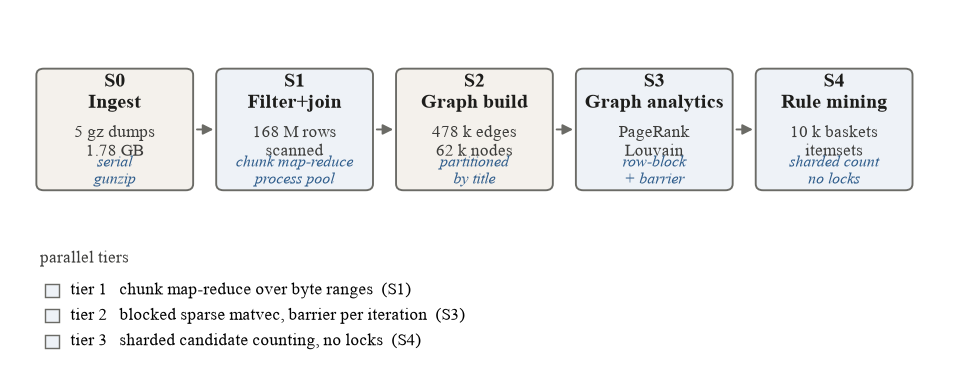
\includegraphics[width=\linewidth]{figures/fig01_pipeline.png}
\caption{Five-stage pipeline. Shaded stages carry a parallel tier; S0 is deliberately serial and is reported as a fixed cost.}
\end{figure}

Decompression deserves a note because it is where a naive design loses the argument. gzip is a single stream: there is no way to seek into it, so the 1.78 GB of compressed input must be expanded by one process into 9.2 GB of text before any parallelism is possible. We therefore measure S0 separately (33.8 s, 4.0\% of the end-to-end serial cost) and exclude it from the speedup computation, rather than hiding it inside a stage boundary. This is the first appearance of a theme that runs through the report: the fraction of a pipeline that cannot be parallelised sets a ceiling on everything that can.

\subsection{Parallel strategy}

The three tiers are deliberately different, because the three workloads stress different parts of the memory hierarchy and have different dependency structures.

\textbf{Tier 1 \textemdash{} byte-range chunk map-reduce (S1, S2).} Each worker takes a contiguous byte range of the uncompressed file, aligned to a newline boundary so no record is split, parses it independently, applies the region filter against a shared read-only set of title identifiers, and returns its filtered rows. The parent merges the partial results. Process-based workers rather than threads were chosen for a specific reason: the stage is parse-bound, and Python's global interpreter lock prevents threads from overlapping parse work, so a thread pool would have produced a flat speedup curve on any number of cores.

Chunk size is a tuned parameter, not a constant. Small chunks improve load balance and keep the working set inside L2/L3, but multiply task overhead and the number of partial results to merge; large chunks reduce overhead but leave cores idle at the tail. Section 4.6 reports the sweep and the selected value.

\textbf{Tier 2 \textemdash{} blocked sparse matrix\textendash{}vector multiplication (S3).} The graph is held as a compressed sparse row matrix of 51,878 nodes and 388,168 undirected edges, symmetrised and row-normalised into a transition matrix. PageRank is then a sequence of sparse matrix\textendash{}vector products, so the question is not how to parallelise it \textemdash{} rows partition cleanly \textemdash{} but how to keep the vector in cache and how much synchronisation each iteration can afford. We implement owner-computes row blocks: the transition matrix is sliced into row blocks once, each worker multiplies its block against the current vector into a private slice of the output, and blocks synchronise only at the iteration boundary. Because each block's output is disjoint, there is no write contention; the only cost is the barrier.

\textbf{Tier 3 \textemdash{} sharded lock-free counting (S4).} Apriori mining has two phases with opposite parallel characteristics. Candidate generation is irregular: the cost of testing a candidate depends on how many baskets contain it, so a static partition produces severe imbalance. Counting is regular: each worker accumulates a local counter over its basket shard and merges once at the end, with no locking inside the scan. Measuring the two phases separately, and showing that the imbalance lives entirely in the first, is the empirical point of Section 4.6.

\subsection{Analysis methods}

\textbf{Centrality.} Degree counts collaborations but conflates prolificacy with importance. PageRank on the undirected, weight-normalised graph corrects for this by propagating importance through the collaboration structure, so a veteran supporting actor who worked repeatedly with leads accumulates rank without topping the degree list. Exact betweenness is O(VE) and intractable here; we use Brandes with k = 64 pivot sources and scale the result, reporting the sampling bias against a k = 256 run.

\textbf{Community detection.} Louvain modularity optimisation provides the primary partition. Because it is stochastic and its output depends on node visiting order, we run it under two random seeds and report normalised mutual information between the two partitions as a stability measure, plus a resolution sweep. Label propagation is implemented as the cheap alternative \textemdash{} it is a single pass per iteration with no global objective \textemdash{} and the modularity gap between the two is reported as a quality/speed trade-off rather than assumed.

\textbf{Temporal profile.} The graph is not re-partitioned per decade; that would make partitions incomparable across slices. Instead labels are fixed from the full graph and, for each bloc, we report the decade distribution of its members' credits, which shows bloc birth, dominance and decline without partition instability.

\textbf{Association rules.} Each film is a basket containing one item per genre plus one item per crew category present in its credits. Itemsets are represented as integer bitsets so that a subset test is a single bitwise AND. Frequent itemsets are mined level-wise to size 3 at minimum support 1\%, and rules are retained at confidence $\geq$ 0.6 and lift > 1.2.

\textbf{Career clustering.} People with at least three credits are described by five features \textemdash{} credit count, number of active decades, peak-decade share, decade breadth, and recency \textemdash{} clustered with k-means, with k selected by silhouette score, and projected to two principal components for display.

\subsection{Evaluation protocol}

Every experiment runs the serial reference and the parallel version over identical input, so that S(p) = T(1)/T(p) compares identical work. Workers p $\in$ \{1, 2, 4, 8, 16\}; each configuration is run and the median reported. Peak resident memory is sampled at 10 Hz over the process tree, so the memory cost of parallelism is reported alongside the time benefit. All timings are on one workstation: 20 logical cores, 32 GB RAM (2 x 16 GB DDR4-4800), Windows 11, Python 3.13.
